\documentclass[border=3pt]{standalone}
% Preâmbulo compartilhado pelos diagramas TikZ da aula 8 de IHR (Métodos de Pesquisa)
\usepackage[T1]{fontenc}
\usepackage[utf8]{inputenc}
\usepackage{lmodern}
\usepackage{amsmath}
\usepackage{xcolor}
\usepackage{tikz}
\usetikzlibrary{arrows.meta,angles,quotes,decorations.pathmorphing,decorations.pathreplacing,calc,
                positioning,shapes.geometric,shapes.misc,backgrounds,fit,
                math}

% Paleta (mesma dos SVGs originais)
% Paleta da disciplina de IHR: acento azul (#1A6FB5), cor de destaque do tema.
% (o nome "dblue" é mantido para não alterar todos os diagramas)
\definecolor{dblue}{HTML}{1A6FB5}
\definecolor{dorange}{HTML}{B3541E}
\definecolor{dgreen}{HTML}{4A7C59}
\definecolor{dred}{HTML}{9C4B4B}
\definecolor{dcream}{HTML}{F4F1EA}
\definecolor{dshade}{HTML}{DDD7C9}

% Função gaussiana (não normalizada por padrão de escala visual)
\pgfmathdeclarefunction{gauss}{3}{%
  \pgfmathparse{1/(#3*sqrt(2*pi))*exp(-((#1-#2)^2)/(2*#3^2))}%
}

% Estilos comuns (prefixo d... para não colidir com chaves internas do pgf)
\tikzset{
  >={Stealth[length=2mm]},
  dguide/.style={gray!55, dashed, line width=0.4pt},
  daxis/.style={gray!60, line width=0.7pt, ->},
  dbody/.style={fill=black!3, draw=black!80, line width=1pt},
  dacc/.style={draw=dblue, line width=1pt},
  dlbl/.style={black!55, font=\small},
  dsub/.style={black!45, font=\footnotesize},
  dstate/.style={circle, draw=black!80, fill=dcream, line width=1pt,
                 minimum size=17mm, font=\large, inner sep=1pt},
  dobs/.style={circle, draw=black!80, fill=dshade, line width=1pt,
               minimum size=14mm, font=\large, inner sep=1pt},
  dbox/.style={rounded corners=2pt, draw=black!80, fill=dcream, line width=1pt,
               align=center, inner sep=6pt},
  dop/.style={circle, draw=black!80, fill=white, line width=1pt,
              minimum size=6mm, inner sep=0pt, font=\small},
  dtrans/.style={->, dblue, line width=1pt},
  dmeas/.style={->, dorange, line width=1pt},
  dcurve/.style={line width=1pt, dblue},
  dcurveb/.style={line width=1.4pt, dorange},
}

\begin{document}
\hyphenpenalty=10000 \exhyphenpenalty=10000 \tolerance=9999 \emergencystretch=3em
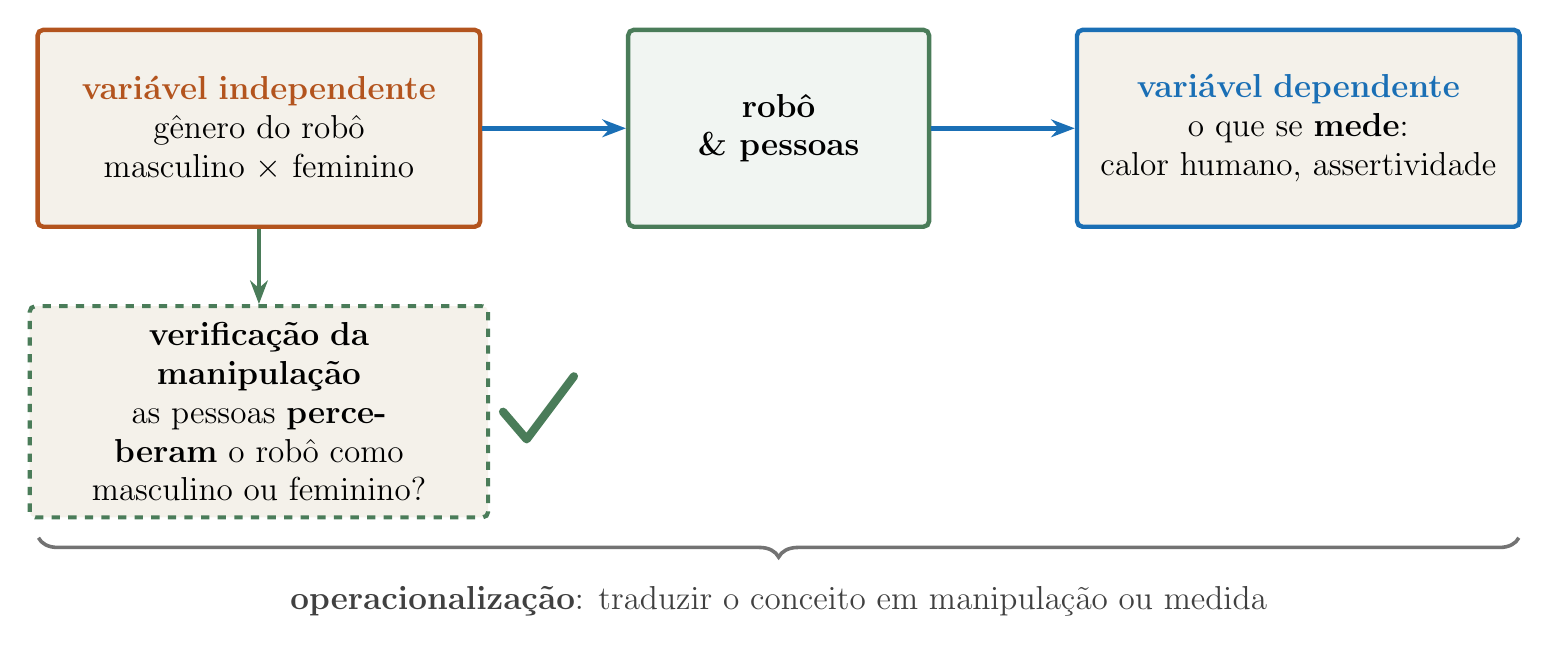
\begin{tikzpicture}[x=1cm,y=1cm]
  \tikzset{b/.style={dbox, text width=5.2cm, minimum height=2.5cm, font=\large, line width=1.6pt, align=center}}
  \node[b, draw=dorange] (vi) at (2.9,5.0) {\textbf{\textcolor{dorange}{variável independente}}\\ gênero do robô\\ masculino $\times$ feminino};
  \node[dbox, draw=dgreen, fill=dgreen!8, line width=1.6pt, text width=3.4cm, minimum height=2.5cm, font=\large\bfseries, align=center] (r) at (9.5,5.0) {robô\\ \& pessoas};
  \node[b, draw=dblue] (vd) at (16.1,5.0) {\textbf{\textcolor{dblue}{variável dependente}}\\ o que se \textbf{mede}:\\ calor humano, assertividade};
  \draw[dtrans, line width=1.8pt, -{Stealth[length=3mm]}] (vi.east) -- (r.west);
  \draw[dtrans, line width=1.8pt, -{Stealth[length=3mm]}] (r.east) -- (vd.west);
  \node[dbox, draw=dgreen, dashed, line width=1.5pt, text width=5.4cm, minimum height=2.3cm, font=\large, align=center] (vm) at (2.9,1.4) {\textbf{verificação da manipulação}\\ as pessoas \textbf{perceberam} o robô como masculino ou feminino?};
  \draw[dgreen, line width=1.6pt, -{Stealth[length=3mm]}] (vi.south) -- (vm.north);
  \draw[dgreen, line width=3pt, line cap=round, line join=round] (6.0,1.4) -- (6.3,1.05) -- (6.9,1.85);
  \draw[black!55, line width=1.3pt, decorate, decoration={brace, amplitude=7pt, mirror}] (0.1,-0.2) -- (18.9,-0.2);
  \node[font=\large, black!75] at (9.5,-1.0) {\textbf{operacionalização}: traduzir o conceito em manipulação ou medida};
\end{tikzpicture}
\end{document}
